\problemname{The Clock}
When someone asks you what time it is, most people respond ``a quarter past five'', \texttt{15:29} or something similar.
If you want to make things a bit harder, you can answer with the angle from the minute hand to the hour hand, since this uniquely determines the time.
However, most people are not used to this way of specifying the time, so it would be nice to have a program which translates this to a more common format.
Your task is to write such a program.

\begin{figure}[h]
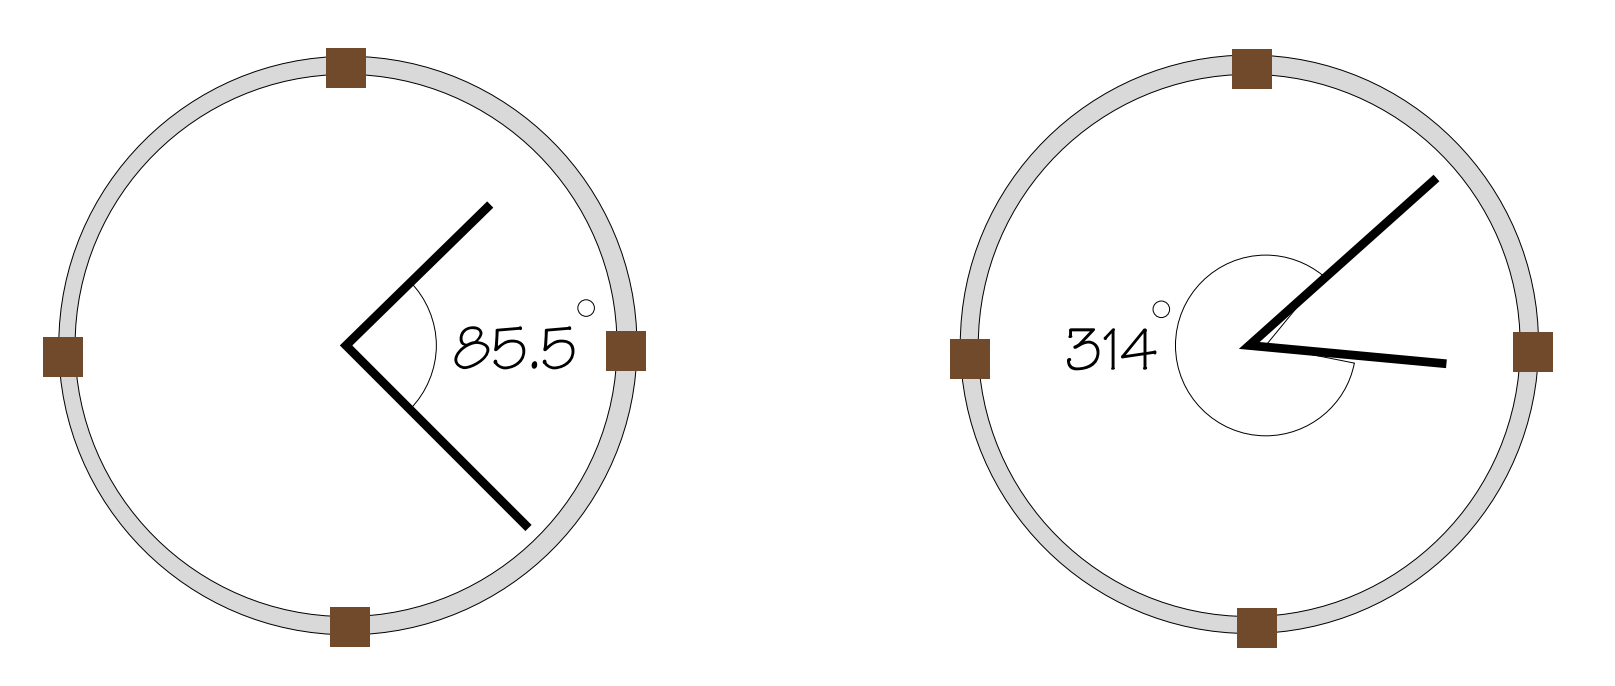
\includegraphics[width=\textwidth]{fig.png}
    \caption{The time on the left is \texttt{01:21}. On the right, it is \texttt{03:08}.}
\end{figure}

We assume that our clock have no seconds hand, and only displays the time at whole minutes (i.e., both hands only move forward once a minute).
The angle is determined by starting at the hour hand and measuring the number of degrees clockwise to the minute hand.
To avoid decimals, this angle is specified in tenths of a degree (so that $85.5$ degrees is written as $855$).
This number is always an integer between $0$ and $3595$ (inclusive) and is, as a consequence of only measuring whole minutes, evenly divisible by $5$.

\section*{Input}
The input consists of a single integer between $0$ and $3595$ -- the angle between the two hands, in tenths of a degree. 

\section*{Output}
Output the time that the angle corresponds to, in the format \texttt{hh:mm}.
We assume that it's morning, so all times should be between \texttt{00:00} and \texttt{11:59}.

\section*{Scoring}
Your solution will be tested on three cases.
The first two gives you $33$ points each, while the last gives you $34$.
